\chapter{Case study}


Case study describes a solution's deployment on the mechanism that was a motivation for this project. The mechanism shown on figures (\ref{fig:mbs} - \ref{fig:render}) is an overconstrainted multibody system (\cite{bib:BPAS2012}), that involves moving platform connected to ground by 6 rigid rods. The lower and upper rods are parallel to each other and have equal length. Although constraints describing the mechanism form a six-dimensional system of equations, they are linear dependent what is observable as a movement of the platform. The mechanism has one degree of freedom, except for two points where a bifurcation occurs. Due to this anomaly it's hard to simplify mechanism model to minimal set of coordinates.

\begin{figure}[!h]
	\centering
	\begin{minipage}{.5\textwidth}
		\centering
		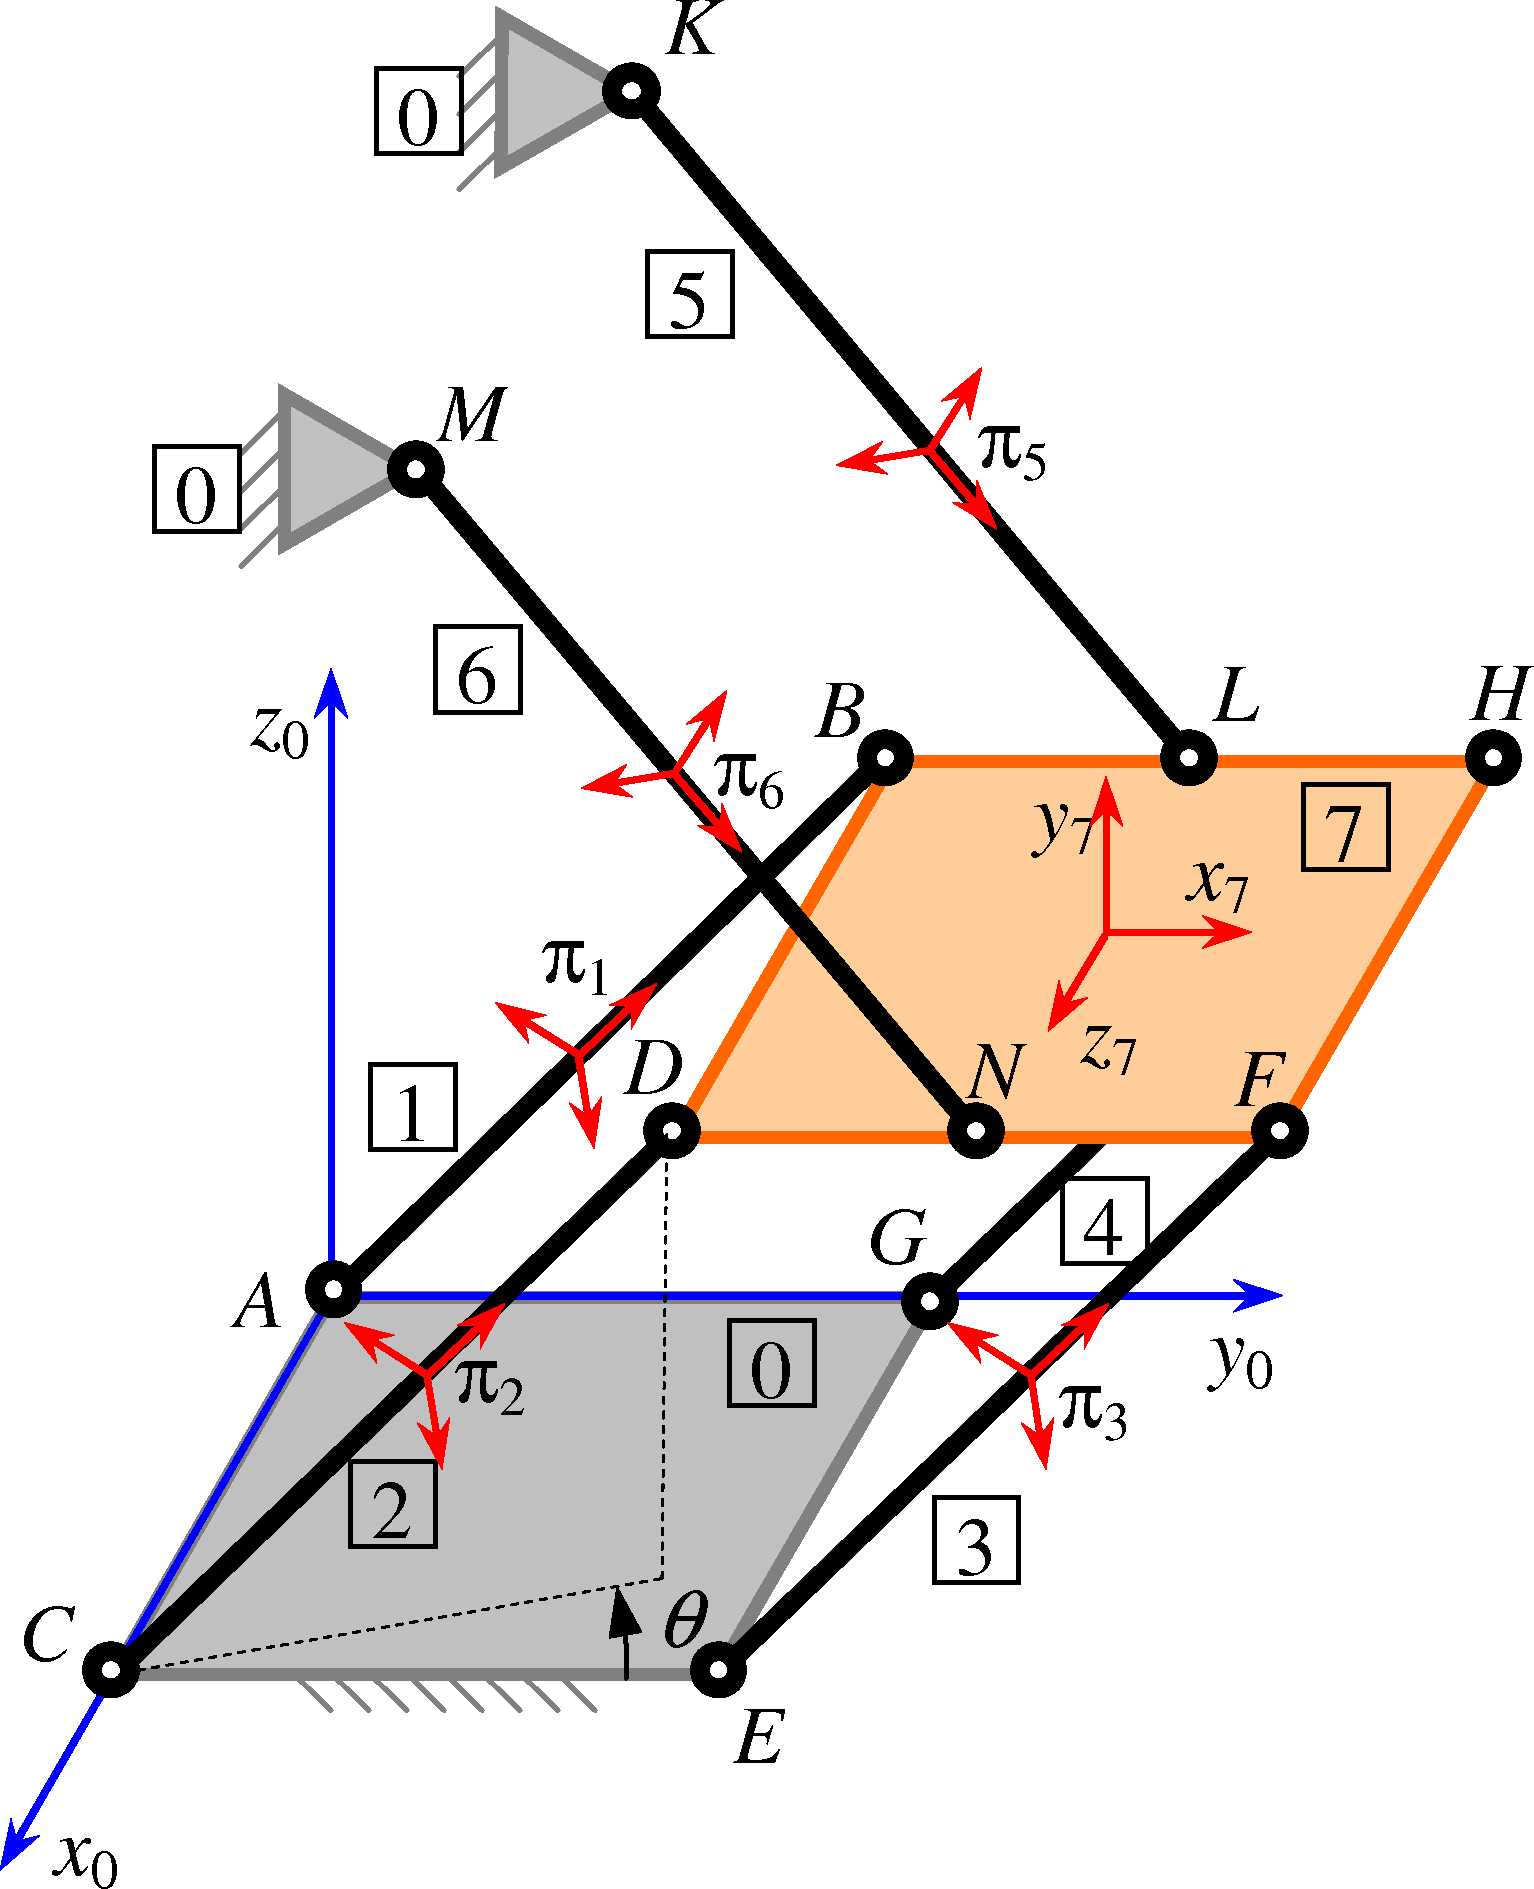
\includegraphics[width=.7\linewidth]{mbs_system.png}
		\captionof{figure}{Multi-body system with 1 DOF}
		\label{fig:mbs}
	\end{minipage}%
	\begin{minipage}{.5\textwidth}
		\centering
		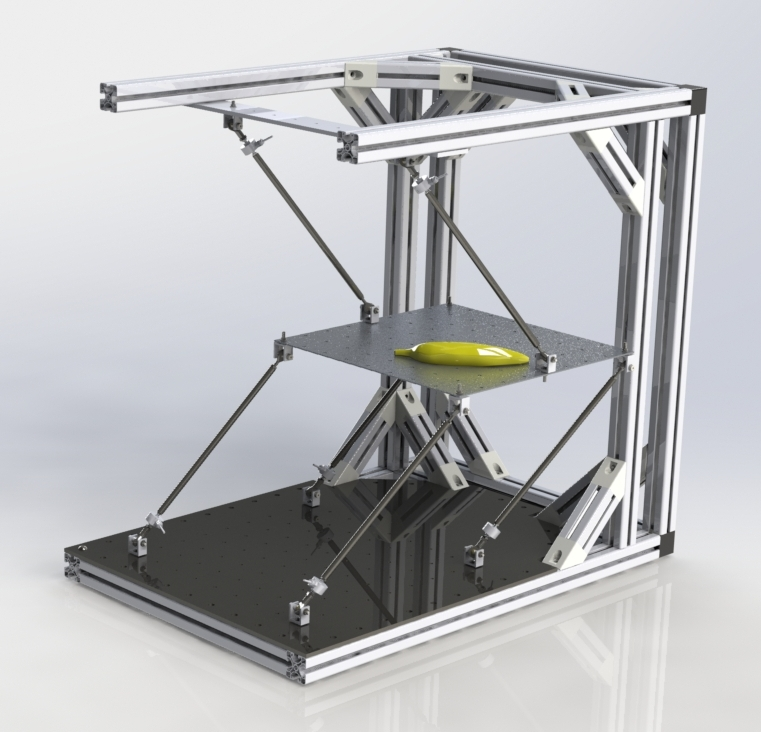
\includegraphics[width=.9\linewidth]{render.jpg}
		\captionof{figure}{Render of MBS}
		\label{fig:render}
	\end{minipage}
\end{figure}

The scientific significance of this mechanism is revealed in the determination of the reaction forces that occur in rods. Mechanism is statically indeterminate which makes it even more difficult to analyze and highlights its research value. The further researches require collecting data from test stand, when the platform moves. State description should contain platform's position and orientation as well as readings from force sensor installed in rods, what is covered by developed system.\\

The mechanism is driven by FANUC M-10iA serial industrial robots. The robot's control system provides arm's tip position. To avoid problems resulting from inaccurate manufacturing the robot is connected to platform center via a drawbar, so the tip's orientation is unusable. Moreover, the position's refresh rate is relatively slow, but can be successfully used in sensor fusion.\\

The mechanism thus presented is a representative example of the application of the developed system. Due to its properties, convetional methods are hard to apply. The proposed solution is challenging as well, but the procedure that lead to working system are structured and split into steps. 

\section{Computer simulation}

Before real-life experiments, the fundamental aspects of projected were tested in computer simulation. The simulation involves preparing kinematic simulation in ADAMS and connecting it with simplified estimation system in MATLAB Simulink. A finished model was used, created earlier as part of a research project. The ADAMS's model was extended with new cylinder-shaped body that represents the robot's tip. The added part is connected with the moving platform's center and will be used as a motion source. A position of the simulated robot's tip is set as a control variable, that input to the program. The kinematic's simulation's outputs are postion and orientation of the moving platform, and its linear acceleration and angular velocity expressed in local coordinates system. Those variables will be used to simulate sensors' readings.
A figure (\ref{adams}) presents multi-body system modeled in ADAMS software. Thus prepared model was converted to a Simulink block. 

\begin{figure}[!h]
	\centering
	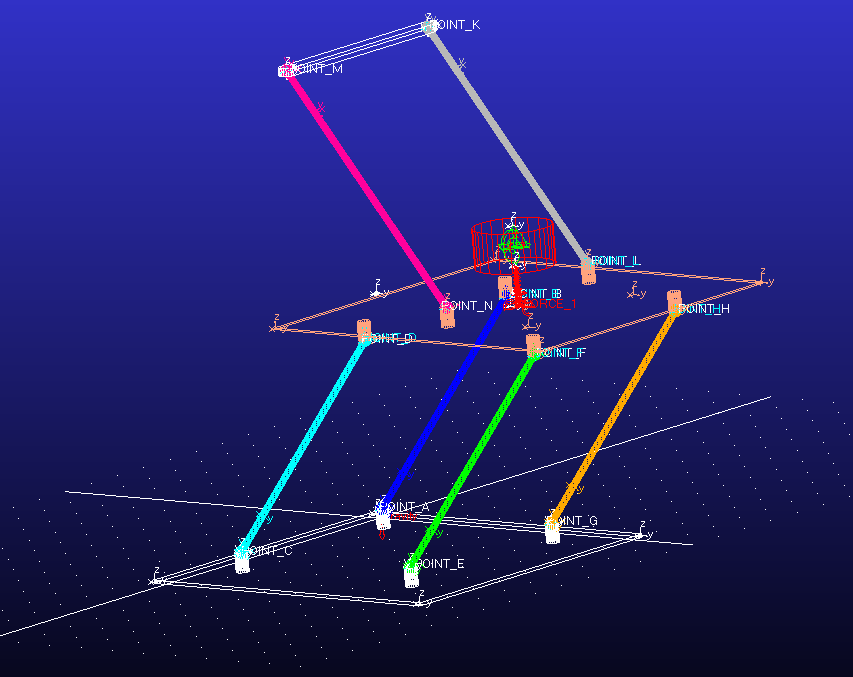
\includegraphics[width=0.8\textwidth]{duw/adams.png}
	\caption{The mechanism modeled in ADAMS software}
	\label{adams}
\end{figure}

Next, to move the mechanism trajectory generator was prepared. One of the allowed trajectory is a circular motion in the horizontal plane. In order to check position tracking the tangential velocity was constantly increased. Equations (\ref{tcp_begin} - \ref{tcp_end}) presents the 3 components of the robot's tip as a function of time.

\begin{align}
	x_{TCP} &= x_0 +  R\ cos( t^2 )
	\label{tcp_begin}\\
	y_{TCP} &= y_0  + R\ sin( t^2 )\\
	z_{TCP} &= z_0
	\label{tcp_end}
\end{align}

With the platform that already moves, the following stage is to simulate inertial sensors: an accelerometer and a gyroscope. The sensors are simulated based on ADAMS block outputs. The gyroscope returns an angular velocity, when the accelerometer returns linear velocity with gravitation acceleration added. A figure (\ref{acc_sym}) presents Simulink blocks that represents an ideal accelerometer.

\begin{figure}[!h]
	\centering
	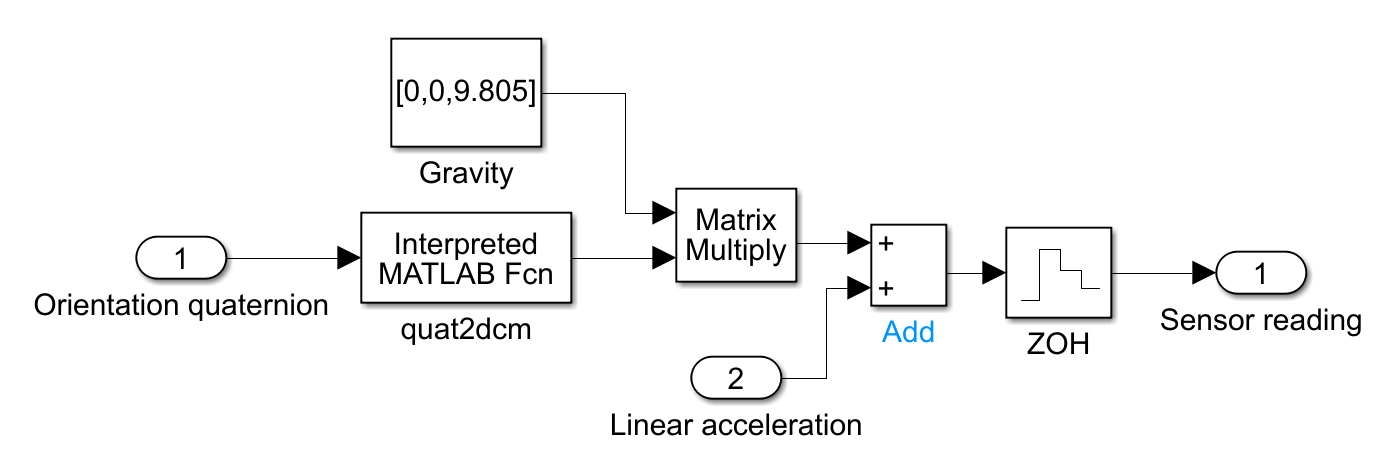
\includegraphics[width=0.7\textwidth]{duw/acc_sim.png}
	\caption{The simulation of an accelerometer}
	\label{acc_sym}
\end{figure}

The outputs of ideal sensors' simulation are further passed to blocks that represents sensor's error. In this simplified simulation the sensor's error was limited to adding a pink noise and bias. A figure (\ref{error_sensor}) presents Simulink blocks that represents a sensor's error.

\begin{figure}[!h]
	\centering
	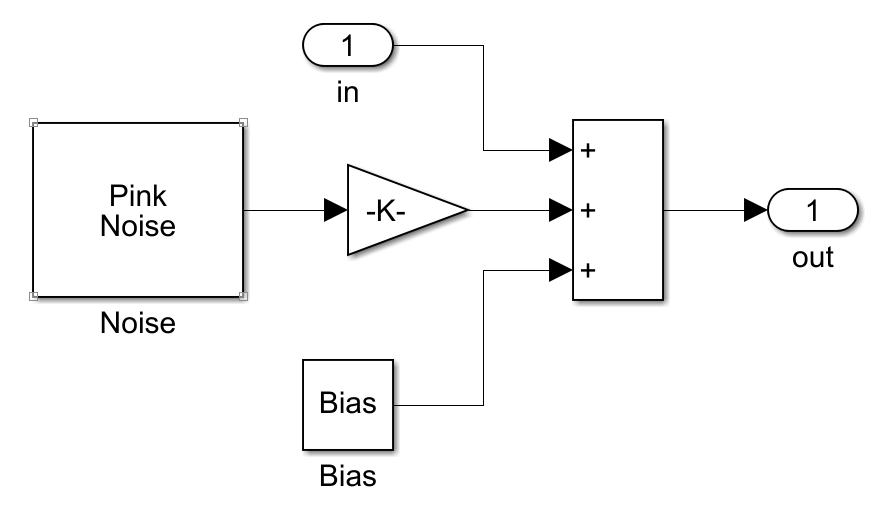
\includegraphics[width=0.7\textwidth]{duw/error.png}
	\caption{The simulation of a sensor's error}
	\label{error_sensor}
\end{figure}

The final step was to implement and tune the Kalman Filter with constraints' correction. Once again, the MATLAB implementation is a simplified version of the filter described in section (\ref{filter_model}). A figure (\ref{ekf_sim}) presents the realization of filter in Simulink MATLAB.

\begin{figure}[!h]
	\centering
	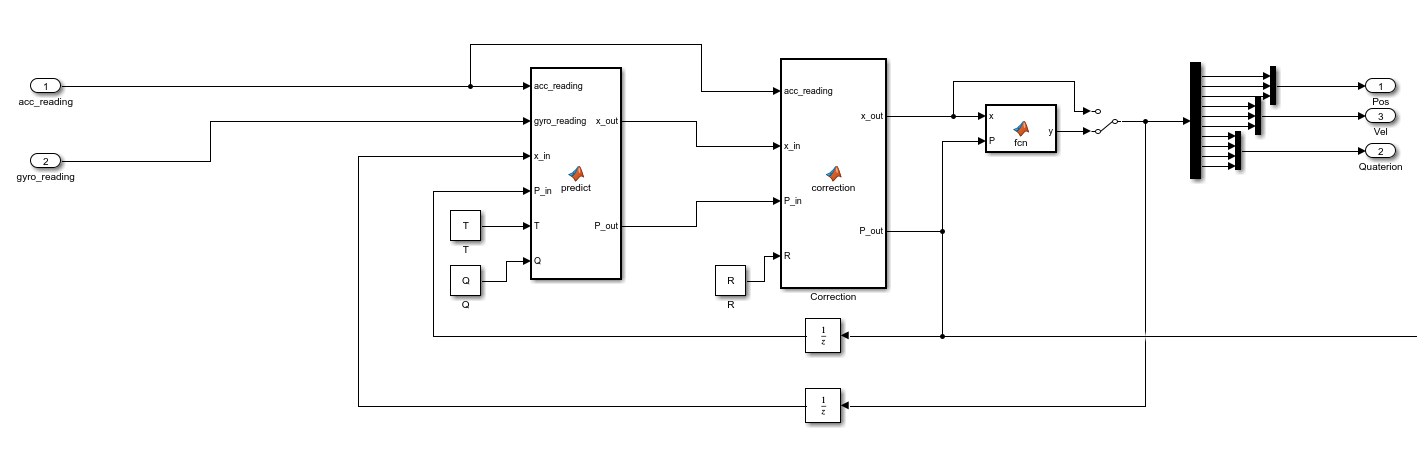
\includegraphics[width=0.9\textwidth]{duw/ekf.png}
	\caption{The Kalman Filter with constraints' correction}
	\label{ekf_sim}
\end{figure}

Thus prepared simulation was run multiple time to select an optimal set of parameters. The presented results are the best achieved after tuning process. First the filter work was examinated without the constraints' correction. A figure (\ref{no_con}) presents the coordinates change in function of time. The plot includes the robot's tip position, the moving platform's center's position and its estimation. The estimation (magenta, yellow and blue colors on plot) drifts heavily over simulation's time.

\begin{figure}[!h]
	\centering
	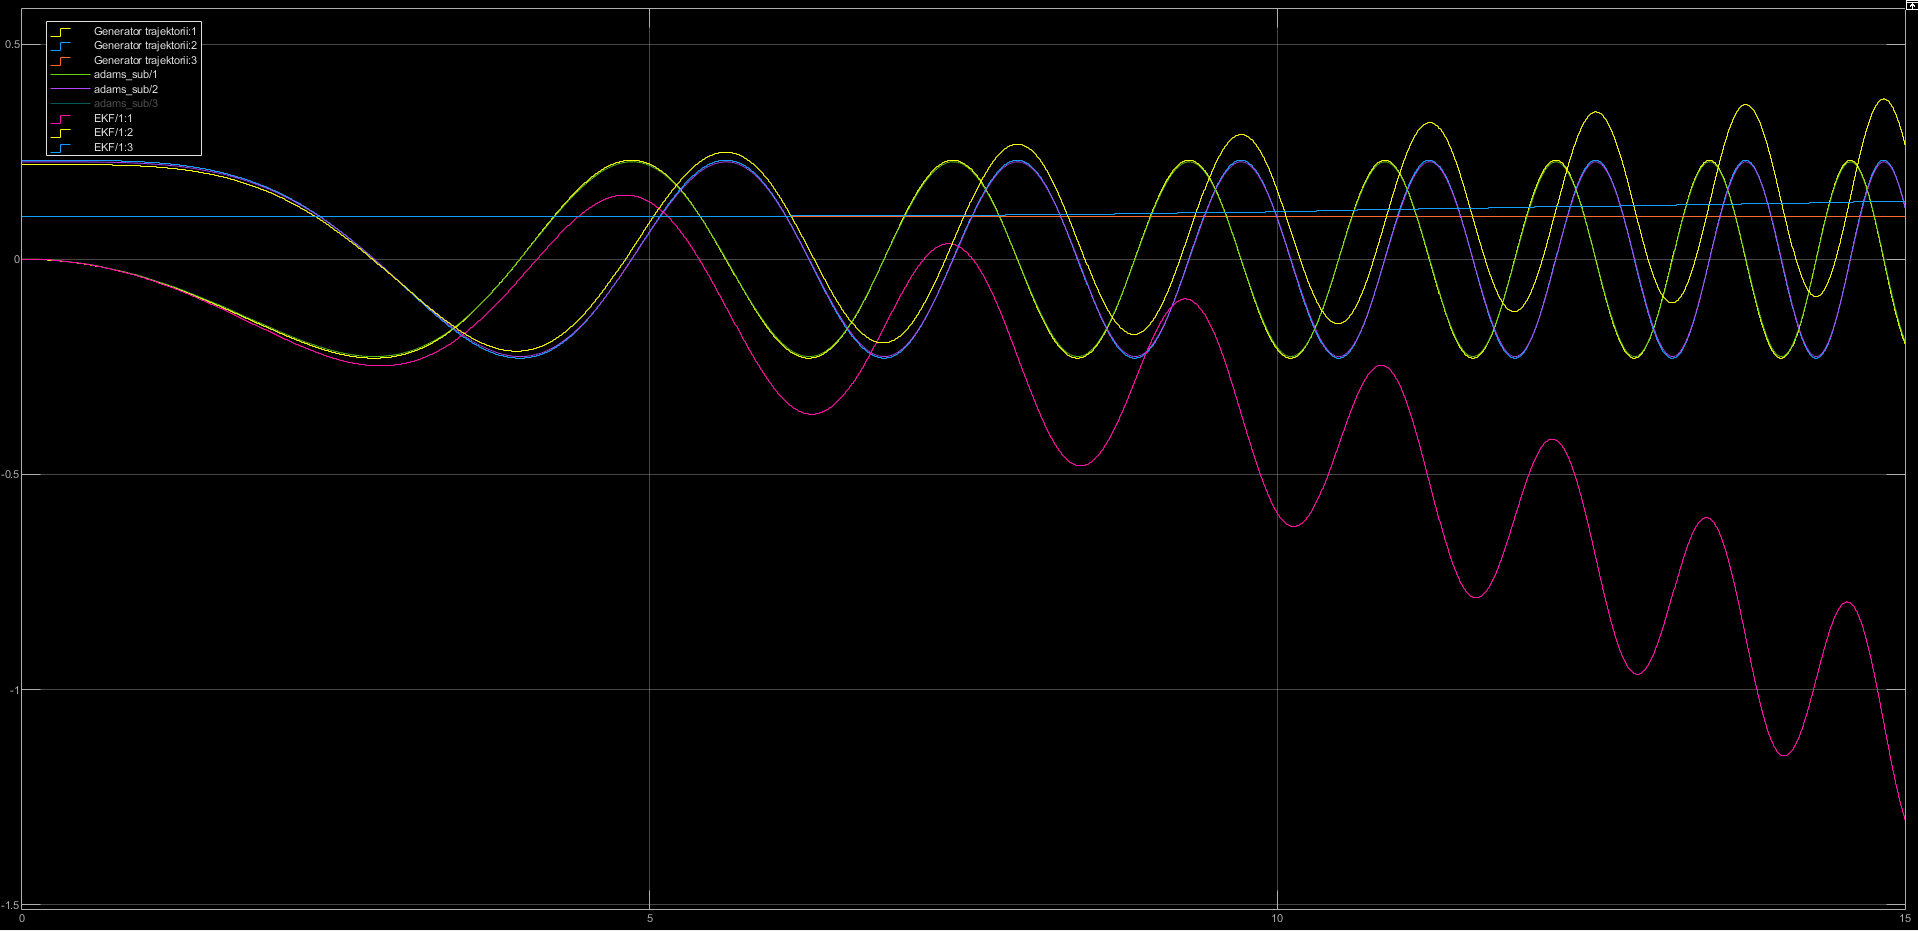
\includegraphics[width=\textwidth]{duw/no_con.png}
	\caption{The result of simulation (no correction)}
	\label{no_con}
\end{figure}

A figure (\ref{corr}) presents the run of same simulation, but with constraints' correction turned on. 
The estimation match the position for most of the simulation. During the second revolution the system lost tracked value but the match was quickly restored.

\begin{figure}[!h]
	\centering
	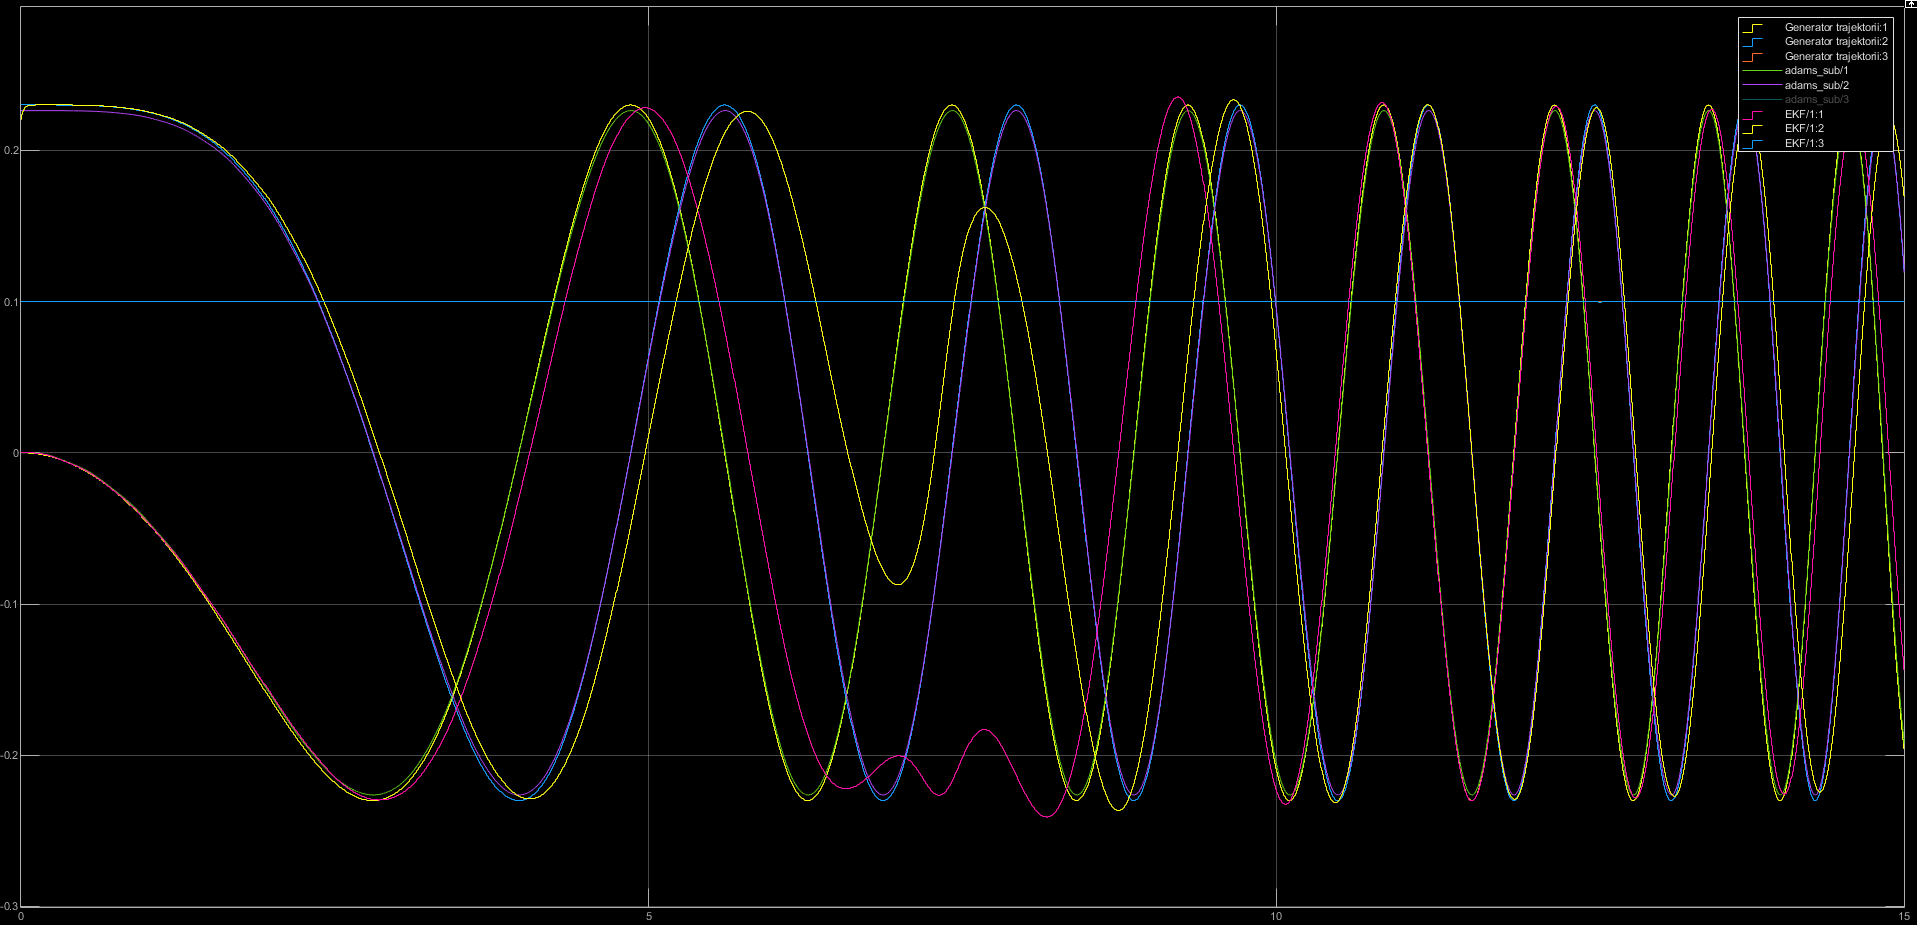
\includegraphics[width=\textwidth]{duw/corr.png}
	\caption{Działanie symulacji z korekty więzów}
	\label{corr}
\end{figure}

\newpage
Summarize, the simulation shows how positive is the impact of using the constraints' correction. The computer simulation was part of preparations for the realization of this work that energized the further work and complete implementation.